\section{Data}
We begin by discussing our data. For now, we only use the 60000 training examples in the {\ttfamily train/} directory. Note that you must extract {\ttfamily train\_LbELtWX.zip} to obtain these examples, as the {\ttfamily train/} directory is deliberately omitted from the repository for performance reasons. These examples are images of 10 classes of apparel, with 6000 examples of each image. Each image is $28\times 28$ and grayscale. We plot some samples of each class in Figure \ref{fig:sampleimages}.

\begin{figure}
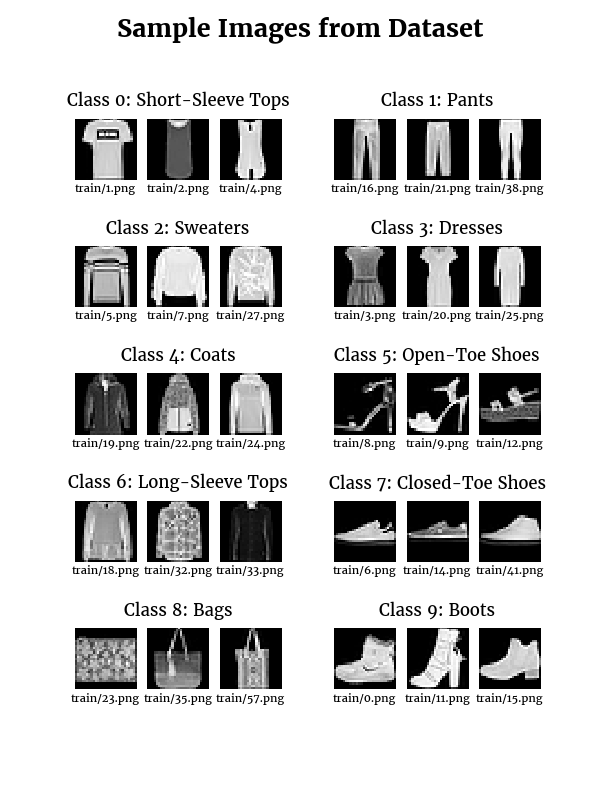
\includegraphics{sample_images.png}
\caption{We present 3 samples from each class of apparel, with predefined class numbers, class names as interpreted by the author, and source files.}
\label{fig:sampleimages}
\end{figure}
\subsection{Basic Analysis}
The dataset here is artificially clean: all the images are centered and upright, with nothing in the background. This should make it easier for our models to classify the data. It also means that some of the advantages of convolutional neural networks over dense neural networks may disappear; however, I still expect that a convolutional neural network will outperform a dense neural network, a belief that has been substantiated by the (undocumented) tests I have run up to this point. Nonetheless, I am training dense neural networks in addition to convolutional networks. I am not doing this because I expect great performance; rather, when I solve computer vision problems with ``messier'' data in the future, I would like to test the hypothesis that dense neural networks will be relatively less effective than in the case of this rather neat dataset.
\subsection{Loading the Data}
The module {\ttfamily load\_data} handles the process of importing data from the {\ttfamily train/} directory. It uses {\ttfamily matplotlib.pyplot.imread()} to load the data, only storing one channel in memory, as the images are grayscale. This will also make it easier to use the GitHub repository. In the future, we can make data loading faster by storing images in grayscale on the drive, preferably in one file; in the dataset, they came as RGB images with three identical channels. When we split the data into training and cross-validation sets in our training scripts, we always use 60\% of the images for training and a random seed of {\ttfamily 1}. Using the same random seed across all tests is critically important, as otherwise there would be no real distinction between our training and cross-validation data.

\subsection{Subdivision of the Classes}
We can see that our classes can be divided into several subgroups that are similar to each other. For example, sweaters and coats may be hard to distinguish, as may boots and close-toed shoes, but footwear can likely be distinguished from outerwear rather easily. While we can most likely get good performance without considering this aspect of our dataset, it may be that there is a way to exploit this concept to save computation time or improve accuracy.

I have not implemented or tested this idea as of yet, and I have no idea whether it would really work, but given that we have a small number of classes, including several subgroups of classes that are similar to each other, I wonder whether the optimal solution may not consist of a single 10-class neural network. Perhaps we could improve performance by first separating into groups of classes (perhaps superclass 0: footwear, superclass 1: tops and dresses, superclass 2: everything else), and then using separate second-level networks to break those apart into the true classes. Potential advantages include (a) the ability to tune the second-level networks independently of each other, and (b) wasting less computation time on relatively trivial distinctions. Potential disadvantages include (i) wasting computation time because the second-level neural networks may recompute features that the first-level network already could have identified, and (ii) overfitting, as the ability to independently tune parameters could make our overall model more complex; (ii) may be partly mitigated by the ability to independently tune image preprocessing and regularization.